\chapter{Object Versioning} \label{chapter:APPROACH}

When programmers unexpectedly introduce problems to the functionality, performance, or design of their applications, they might want to recover a previous development state.
In programming systems like Lively, where programmers often work at runtime on objects, a development state consists of objects, or, more precise, of the state of objects, which includes object-specific behavior.
To be able to recover such a development state, comprehensive recovery support for Lively must, therefore, preserve versions of objects.

Our approach for this builts upon alternative, version-aware references that manage versions of objects transparently.
That is, objects are pointed to through references that dynamically and transparently choose versions of objects as they were at a particular moment.
When these references are then used for all mutable objects of a runtime, the entire runtime state can be preserved and re-established.

Our concrete solution for implementing this in JavaScript and for the Lively Kernel relies on proxies and source transformations.
Using proxies and source transformations allows a language-level solution for alternative references.
The proxies, in this solution, also contain the versions of the object they stand-in for, enabling the ordinary JavaScript garbage collection to reclaim the versions of an object when the version-aware reference is no longer used.



\section{Version-aware References} \label{sec:APPROACH:1}

For object versioning in systems like Lively, we propose alternative, version-aware references to manage multiple versions of objects.
These version-aware references know the available versions for an object and resolve to one of those.
A version of an object is, in the simplest case, a copy of an object---also an object and also part of the application memory.
That is, a version-aware cencapsulates the multiplicity of different objects for conceptually the same object.

To preserve complete development states, all objects of the programming runtime need to be preserved and accessed via version-aware references.
That is, to save a version of the runtime, versions of all objects are preserved---which also entails that the side effects to the state of other programs, for example server processes, or to databases are not preserved with this approach.
To then re-establish a version of the runtime, the version-aware references all choose versions of objects that were preserved together.
This way, multiple version-aware references can be resolved transitively to the state as it was when the versions were preserved.

Version-aware references behave transparent, like usual references.
They can be assigned to variables and be passed around, and, under usual circumstances, programmers do not have to be aware of them.
Firstly, programmers should not have to adapt their program code to use version-aware references.
Instead version-aware references should be provided consistently by the programming system.
Secondly, there should not be direct references to particular versions of an objects, which otherwise would potentially introduce inconsistencies.
Programmers should not have to distinguish between version-aware references and direct references.

This approach to object versioning allows incremental versioning, without interrupting the system.
The version-aware references resolve dynamically to particular versions based on context information.
Only this context information has to be changed to have all references resolve to another version, without updating any of the version-aware references.
Similarly, preserving a new version of the runtime can also happen incrementally.
Instead of preserving versions of all objects that make up the runtime, new versions of objects are only created when objects change.
Before writes, the previously preserved objects continue to reflect the current state and can, thus, be read for following versions.
This way, versioning happens on the granularity of objects.

\begin{figure}[h]
    \centering
    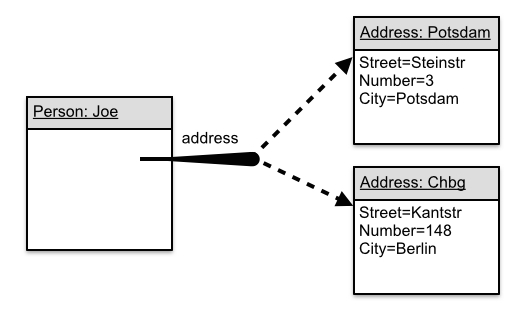
\includegraphics[width=0.5\textwidth]{figures/versionAwareReference.png}
    \caption{A Person object with two versions for its address.}
    \label{fig:VersionAwareReference}
\end{figure}

Figure~\ref{fig:VersionAwareReference} shows a version-aware reference and three objects:
a \emph{Person} object and two different versions of conceptually the same \emph{address} object.
The person holds the version-aware reference to the addresses in its \emph{address} slot.
The version-aware reference can resolve to both, dynamically using context information to decide this matter.
That is, it does not have to have one of the versions hard-wired as active version.

\begin{figure}[h]
    \centering
    \includegraphics[width=\textwidth]{figures/MultipleVersionAwareReferences.png}
    \caption{Three versions visible in the version-aware references of a simple object graph.}
    \label{fig:MoreVersionAwareReferences}
\end{figure}

To resolve entire object graphs to consistent versions and as they have been at particular moments, versions of objects are created and resolved in a coordinated way.
For this example, we assume that the context information that is used to resolve version-aware references, is a global version identifier that corresponds to meta-information stored in the version-aware references, as shown in Figure~\ref{fig:MoreVersionAwareReferences}.
This example shows a slightly more comprehensive graph that might result from preserving specific versions while changing particular objects.
We have an initial version, \emph{v1}.
In this, a \emph{Company} object is created and that refers to a \emph{CEO} object using a version-aware reference.
The CEO in turn has an address, also referred to via a version-aware reference.
Next, we preserve this version and then, in version \emph{v2}, the same CEO moves to Berlin.
Therefore, the version-aware reference to the address of the first CEO knows two different addresses.
Finally, to achieve the situation as shown in the figure, we preserve the second version and, in version \emph{v3} change the company's CEO and this new CEO has its own address.
Now, given the knowledge that \emph{v3} is preceded by \emph{v2} and that by \emph{v1}, the version-aware references can resolve to three different development states the runtime was in.
When, for example, changing the CEO turns out to be a mistake, we can re-establish \emph{v2} and, therefore, the old CEO with its address in Berlin.
This way, when version-aware references are used consistently for all object relations in a programming runtime, the state of the entire runtime can be set to particular versions.

What versions of the runtime get preserved is not inherent to our approach, but can be different for different use cases.
Programmers could, as described in the second example, explicitly preserve versions or the programming system could implicitly preserve versions.
For example, each manipulating user interaction could yield a new version of the runtime.
Such actions could include directly manipulating attributes and composition of graphical elements, saving source code, evaluating do-its, and, for example, firing buttons of applications.
This way, programmers could undo each of their actions, regardless of whether the action was intended as mere exploration or turned out inappropriate more unexpectedly.
Using user actions as granularity also allows developers to undo and redo the changes associated with specific and rememberable actions.
The resulting histories can be fine-grained as for each version only changed objects need to be copied.
For the same reason, creating many versions is not expected to be problematic for the development workflow.
In general, the approach distributes the cost for object versioning: besides incrementally saving a version, switching the active version is also not interruptive.
Switching the active version is also inexpensive due to the fact that all versions of objects and, thus, all versions of the runtime are kept in the application memory.


\section{Object Versioning for the Lively Kernel} \label{sec:APPROACH:2}

Our approach for providing object versioning in JavaScript, built in and for the Lively Kernel, uses proxies to implement version-aware references.
Instead of accessing mutable objects directly, proxies are accessed.
In fact, our implementation exchanges ordinary references to objects with references to proxies, which then manage and delegate to different versions of the objects.
This exchange is accomplished by returning proxies whenever a new object is created.
For this, sources are transformed to proxy object literals and any constructor functions.
Further, the proxies return proxies when they are used as constructors.
Also, through proxy behavior and some global versioning management, we provide basic recovery support---simple undo and redo---for the single-threaded Lively Kernel programming system.


\subsection{Proxies as Version-aware References}

Proxies allow a language-level implementation of alternative references in JavaScript:
Without requiring adaptions to the virtual execution engines, proxies can be inserted to stand-in for objects---so references that usually point directly to objects point to proxies instead---and these proxies can provide versioning information and behavior.
These proxies are then an alternative to using ordinary references directly to point to objects.
That is, some objects can, potentially, still be referred to directly, while state that should be preserved should be proxied.
In our solution for Lively, nearly all objects are only accessed through proxies, except for some particular \emph{root objects} that are not required to be versioned but do refer to other objects via version-aware references.

The proxies required for our solution are virtual-object proxies, not associated especially with a particular version of an object.
Instead when such a fully virtual object proxy is created for an object, the original object is just taken as one version, the inital version.
The proxies then need to be able to intercept and arbitrarily handle all kinds of access transparently.
In fact, the proxies need to fulfill at least three responsibilities:
\begin{enumerate}
    \item They need to know which versions are available for a particular object.
    \item They need to choose one particular version among all available dynamically according to context information.
    \item They need to delegate object access transparently to a chosen version.
\end{enumerate}

In our solution, we used the proxy objects also to hold all versions of the object they stand-in for.
This way, when the proxy is no longer reachable and, thus, eventually garbage collected, all versions of the objects are also collected.
For example, in the following code snippet, there would temporarily exist a version-aware reference---a proxy---connecting the \emph{Person} object to an \emph{Address} object, but the reference gets deleted before a version of the person is preserved.
Thus, nothing prevents the garbage collector from claiming the proxy for the address object right with the single existing version of it.
\iffalse
\begin{verbatim}\fi
\begin{code}[lst:example]{}{float,numbers=left}
    var person = {name: "Lauritz"};
    \\ preserve version
 person.currentAddress = {street: "Friedrichstrasze",
                         number: "112b",
                         city: "Berlin"};
    delete person.currentAddress;
    \\ preserve version
\end{code}
\iffalse
\end{verbatim}\fi
% person.currentAddress = {street: % "Friedrichstraße",
%                         number: % "112b",
%                         city: % "Berlin"};
This way, starting from each root object, the version-aware references span a graph with potentially multiple available versions for each object, required to follow different paths that correspond to different versions of the graph.



\subsection{Proxies For All Mutable Objects}

% This ensures that references to proxies are used consistently instead of direct references to objects and that such proxies are used for every object.

When proxies are supposed to provide a kind of alternative references, ordinary references that usually point directly to an object now need to point to an object's proxy instead, which then can refer to one or multiple versions of the object.
To have all references refer to proxies instead of actual objects, proxies are created and returned for each new object.
The only reference to the actual object---or, more precisely, the initial version of an object---remains inside the proxy, while the reference to the proxy gets passed around instead.
Therefore, all access goes through the proxy and it can ensure that a particular version of an object is used.
Also, all references that would usually point to the same object now point to the same proxy, which, thereby, provides object identity.
Checks that would usually compare the object with potentially other objects now compare the proxy with potentially other proxies.

For this solution, all expressions that create new objects need to return proxies for those instead.
In JavaScript, there are three different ways to create an object: 
\begin{itemize}
    \item evaluating literal expressions: e.g. \lstinline|{age: 12}|
    \item applying constructor functions: e.g. \lstinline|new Person(12)|
    \item calling specific built-in functions: e.g. \lstinline|Object.create(prototype, {age: 12})|
\end{itemize}

We use source transformations to wrap literal expressions consistently into a \emph{proxy} function.
That function takes an object as parameter and returns a proxy for that object.
Besides objects arrays and functions are also mutable objects in JavaScript.
Therefore, we wrap the literal forms of objects, arrays, and functions.
For exampe, \lstinline{[aPerson, aCompany]} becomes \lstinline{proxyFor([aPerson, aCompany])}.

In JavaScript, all functions can be constructors and create new objects when called with the \emph{new} operator.
Functions expressed as function literals already get proxied with the previous source transformations and the proxies we use for version-aware references intercept different object access differently.
That is, proxies for functions can have constructor behavior that always returns proxies for newly created objects.

For the functions that create new objects but are built-in and, thus, are not created from literal form, the transformation of literals and proxy behavior is not enough.
One category of such built-in functions are built-in constructors.
For example, the built-in data types like objects and arrays can be created by calling \lstinline{new Object()} or \lstinline{new Array()}.
We transform these built-in constructor functions explicity, wrapping each into the proxying function.
Besides these built-in constructors, there are also very specific built-in functions, that we transform separately to specific alternatives.
One example for such functions is the global eval function.
While the return value of that function also potentially needs to be a reference to a proxy instead of an ordinary object, eval takes arbitrary code which might express an arbitrary object structure and which might require multiple references to point to proxies.
Therefore, in the specific case of eval, we proxy eval's result, but also let the string argument to the eval function pass through the source transformations beforehand.

\subsection{Versions of the Lively Runtime} % how the proxies / version-aware references now allow to switch and create versions of the runtime.

Proxies hold multiple versions of an object.
They can transparently delegate access to one particular amony many versions.
They are also referred to consistently instead of the object.
This allows to have and use particular versions of particular objects.
However, to enable programmers to undo and redo arbitrary changes to the entire development state, our solution needs to preserve and choose versions of all objects in a coordinated way.
Our solution to this is declaring versions of the runtime, preserving relationships between those versions, and annotating versions of objects with the version of the runtime they are part of.

Our proxies hold available versions of an object and associate each version of the object with the version of the runtime it belongs to.
When a proxy is created for an object, the object is preserved as the version of the object that belongs to the current version of the runtime.
On writes, the proxies copy the latest version of the object and then do the write on the copy instead.
The copy gets marked with the identifier of the new version of the runtime.
When the proxies now choose a particular version of the object they stand-in for, they all use the version associated with the current version of the runtime or of a previous versions.
This way, the proxies transitively all delegate to objects that accurately represent the state of the entire runtime as it was at a particular moment---when the version of the runtime was last active.
To preserve a development state, the version of the runtime just has to be changed.

The version of the runtime can be global in JavaScript as JavaScript engines use only a single thread and cooperative scheduling.
There is, therefore, no way to change which version of each object should be used while a path through an object graph is already partly resolved.
The version also may have a predecessor and a successor.
This way, for undo and redo the current version of the runtime only has to be set on the predecessor or the successor.
Preserving the predecessor also allows to preserve versions of objects only on writes as, when objects have not changed in versions, the first available previous version of the object can be read.

% Besides this copy-on-write optimization, another optimization would be to not copy objects completely, but to only store changes.
% this could, for example, also apply prototypical inheritance to have versions that delegate to previous versions and only express the differences between versions.

% further, as the proxies already hold all versions, they also create new versions of objects in our solution, copies, when indicated by the programming system.
